\documentclass[12pt]{article}
  \usepackage{geometry}
  \geometry{
    a4paper,
    total={170mm,257mm},
    left=20mm,
    top=20mm,
  }
%Packages
\usepackage{polski}
\usepackage[T1]{fontenc}
\usepackage[utf8]{inputenc}
\usepackage{color}   
\usepackage{listings}
\usepackage{graphicx}
\usepackage{float}
\usepackage[hidelinks,linktoc=all]{hyperref}
\usepackage{hyperref}
\usepackage{amsmath}


% listings definition
\definecolor{dkgreen}{rgb}{0,0.6,0}
\definecolor{gray}{rgb}{0.5,0.5,0.5}
\definecolor{mauve}{rgb}{0.58,0,0.82}
\definecolor{purple}{rgb}{0.41, 0.16, 0.38}
\lstdefinelanguage{JavaScript}{
  keywords={break, case, catch, continue, debugger, default, delete, do, else, false, finally, for, function, if, in, instanceof, new, null, return, switch, this, throw, true, try, typeof, var, void, while, with},
  morecomment=[l]{//},
  morecomment=[s]{/*}{*/},
  morestring=[b]',
  morestring=[b]",
  ndkeywords={class, export, boolean, throw, implements, import, this},
  keywordstyle=\color{blue}\bfseries,
  ndkeywordstyle=\color{gray}\bfseries,
  identifierstyle=\color{black},
  commentstyle=\color{purple}\ttfamily,
  stringstyle=\color{red}\ttfamily,
  sensitive=true
}
\lstset{language=Java,
  basicstyle={\small\ttfamily},
  belowskip=3mm,
  breakatwhitespace=true,
  breaklines=true,
  classoffset=0,
  columns=flexible,
  captionpos=b,   
  commentstyle=\color{dkgreen},
  framexleftmargin=0.25em,
  frameshape={}{yy}{}{}, %To remove to vertical lines on left, set `frameshape={}{}{}{}`
  keywordstyle=\color{blue},
  numbers=none, %If you want line numbers, set `numbers=left`
  numberstyle=\tiny\color{gray},
  showstringspaces=false,
  stringstyle=\color{mauve},
  tabsize=3,
  xleftmargin =1em
}

% images adding definition
\graphicspath{ {img/} }
\newenvironment{centerfig}
{\begin{figure}[H]\centering}
{\end{figure}}

\begin{document}

% Headings
\title{Internet Rzeczy}
\author{
  \textit{AGH, Wydzial Informatyki Elektroniki i Telekomunikacji} \\ \\
  \textbf{Dzmitry Mikialevich}\\
  \textbf{Kinga Sąkól}\\
  \textbf{Imie Nazwisko}\\
  \textbf{Imie Nazwisko}\\
  \textbf{Imie Nazwisko}\\ \\
  \textbf{BlockChain}
}
\date{ }
\maketitle
\tableofcontents

\newpage

\section{Możliwe Tematy}
% TODO Delete this section
1. Wprowadzenie do tematu block-chain: czym się różni od systemów rozproszonych? Jakie ma wady i zalety?
2. Obszary zastosowań block-chain, w tym: czy możemy za pomocą danej technologii określić wiarygodność danych,
na których pracujemy? Czy w przypadku np. uszkodzenia sensora moglibyśmy cofnąć się na tyle, żeby określić, w którym momencie dane jeszcze nie były zaburzone?
3. Możliwość implementacji danej technologii: jakie są wymagania? Czy istnieją pewne biblioteki albo narzędzia, ułatwiające implementację?
4. Przegląd artykułów, związanych z danym tematem. Dostęp do artykułów możemy uzyskać za pomocą biblioteki głównej AGH. Szczególnie przez Pana Doktora zostało polecone przeglądnięcie IEEE Xplore na stronie http://www.bg.agh.edu.pl/pl/vezrodla/I
Muszą być sprawdzone 5-10 artykułów na ten temat.
5. Przegląd istniejących w tej chwili produktów oraz projektów na Github - czy w danej chwili są jakieś start-up`y, związane z daną technologią? Czy istnieje możliwość zakupu takich produktów? Kod nie jest potrzebny, tylko analiza, może jakaś tablica, wykresik itd.

\section{Wprowadzenie do tematu blockchain}

Wprowadzenie do tematu block-chain: czym się różni od systemów rozproszonych? Jakie ma wady i zalety?

\subsection{Systemy rozproszone}

\textbf{System rozproszony} to system, którego komponenty znajdują się na różnych komputerach w sieci, które komunikują się i koordynują swoje działania, przekazując sobie nawzajem wiadomości \cite{wiki-sr}. \\
Istotne cechy systemów rozproszonych, to współbieżność komponentów, brak zegara globalnego i niezależna awaria komponentów. \\
Powyższe pozwala na zdecentralizowanie systemu, który jest zbudowany na komputerach w sieci. Co pozwala na zwiększenie bezpieczeństwa oraz niezawodności takiego systemu.\\
Jedną z możliwych technologji systemów rozproszonych jest Technologia rozproszonego rejestru (DLT). \\
\subsection{Technologia rozproszonego rejestru (DLT)}
Technologia rozproszonego rejestru (również „Technologia rozproszonych rejestrów”, ang. Distributed Ledger Technology, DLT) - technologia rozproszonej bazy danych, której rejestry są replikowane, współdzielone i zsynchronizowane w ramach konsensusu różnych, rozproszonych geograficznie, osób, firm lub instytucji. \cite{wiki-dlt}

W odróżnieniu od systemów zcentralizowanych nie ma centra przetwarzania danych oraz administratora centralnego.

Informacja jest przechowywana w node'ach, każdy z których zawiera pełną kopię informacji w blokach zgodnie z czasem dodania.

\begin{centerfig}
  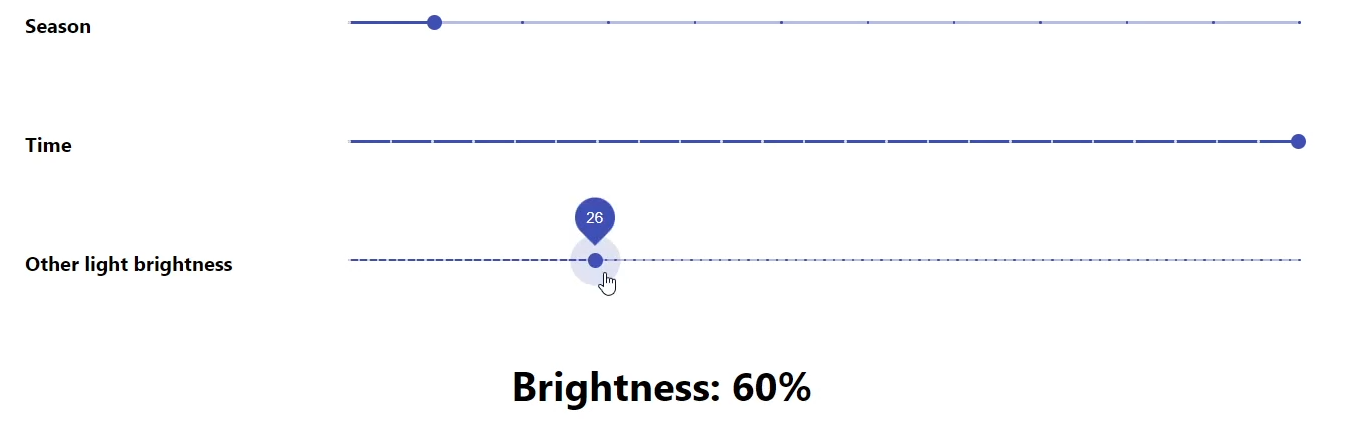
\includegraphics[width=\textwidth]{1.png}
  \caption{Różnica między systemem rozproszonym a systemem zcentralizowanym \cite{sceta}}
\end{centerfig}

Podstawową zaletą jest decentralizacja. Gdy nastąpi aktualizacja "księgi", każdy węzeł konstruuje nową transakcję, a następnie węzły głosują według algorytmu konsensusu, który egzemplarz jest poprawny. Po ustaleniu konsensusu wszystkie inne węzły aktualizują się nową, poprawną kopią księgi.\\
Bezpieczeństwo osiąga się za pomocą kluczy kryptograficznych i podpisów.

\begin{centerfig}
  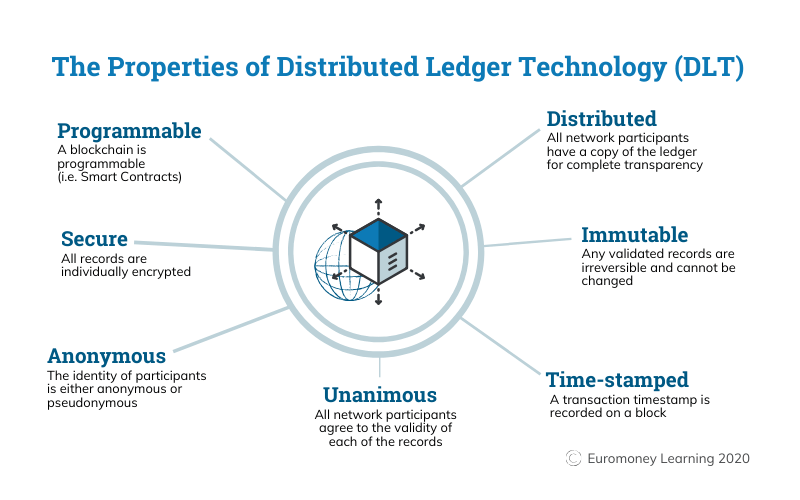
\includegraphics[width=\textwidth]{2.png}
  \caption{Własności DLT\cite{2png}}
\end{centerfig}

\subsection{Blockchain}

Blockchain to rozproszona baza danych (DLT), która jest współużytkowana przez węzły sieci komputerowej.

\begin{centerfig}
  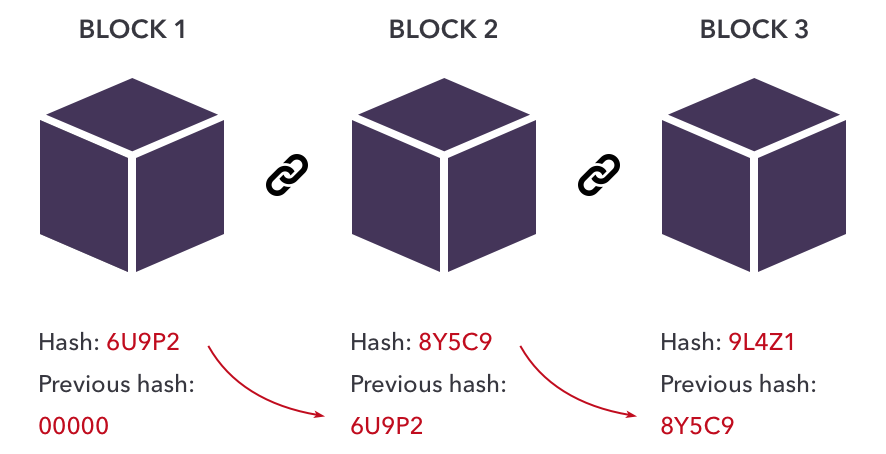
\includegraphics[width=\textwidth]{3.png}
\end{centerfig}

Blockchain to rosnąca lista rekordów, zwanych blokami, które są połączone ze sobą za pomocą kryptografii. Każdy blok zawiera skrót kryptograficzny poprzedniego bloku, znacznik czasu i dane transakcji (zazwyczaj reprezentowane jako drzewo Merkle). \\
Znacznik czasu dowodzi, że dane transakcyjne istniały w momencie publikacji bloku w celu dostania się do jego hasha. Ponieważ każdy blok zawiera informacje o bloku poprzedzającym, tworzą one łańcuch, a każdy dodatkowy blok wzmacnia bloki przed nim. Dlatego łańcuchy bloków są odporne na modyfikację swoich danych, ponieważ raz zarejestrowane dane w dowolnym bloku nie mogą zostać zmienione wstecznie bez zmiany wszystkich kolejnych bloków. \cite{wiki-blockchain}

Blockchainy są najbardziej znane ze swojej kluczowej roli w systemach kryptowalut, takich jak Bitcoin, w utrzymywaniu bezpiecznego i zdecentralizowanego rejestru transakcji. Innowacja w Blockchain polega na tym, że gwarantuje wierność i bezpieczeństwo rejestru danych oraz generuje zaufanie bez potrzeby korzystania z zaufanej strony trzeciej.

% TODO Proof of work
% TODO Some cleaning and rewriting


\subsection{Czym się różni Blockchain od systemów rozproszonych i DLT}

Blockchain to jedna z możliwych implementacji systemów DLT (które wówczas są systemami rozproszonymi). DLT nie wymaga od nas sekwencji bloków oraz użycia koncepcji "proof of work".

\subsection{Wady i zalety blockchaina}

\subsubsection{Wady}
\begin{itemize}
  \item Nie idealnie bezpieczny (wystarczy >50\% "node influence")
  \item Nie energooszczędny
  \item Brak centralizacji powoduję problemy (np. przy utracie klucza prywatnego, albo zapobieganie działaniam nielegalnym)
\end{itemize}

\subsubsection{Zalety}
\begin{itemize}
  \item Szybsze transakcję
  \item Większe bezpieczeństwo
  \item Decentralizacja
\end{itemize}

\section{SectionName}

% Insert images
\begin{centerfig}
  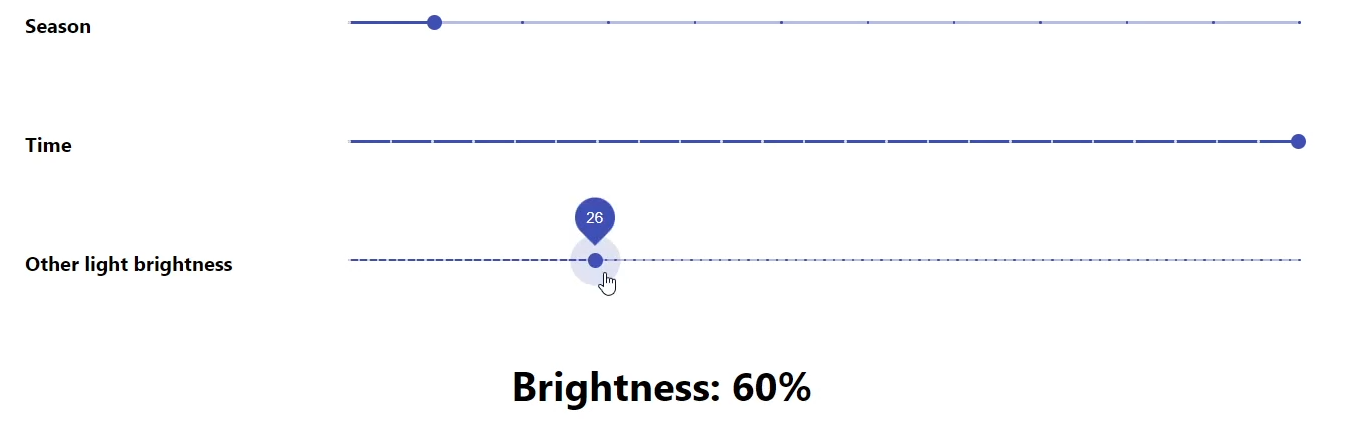
\includegraphics[width=\textwidth]{1.png}
\end{centerfig}

\section{Obszary zastosowań blockchain, w tym: czy możemy za pomocą danej
technologii określić wiarygodność danych, na których pracujemy? Czy w przypadku np. uszkodzenia sensora moglibyśmy cofnąć się na tyle, żeby określić, w którym momencie dane jeszcze nie były zaburzone?}

\subsection{Obszary zastosowań blockchain}
\subsubsection{Finanse}
Instytucje finansowe przeprowadzają interesy z klientami przestrzegając określonych procedur, które często są dość skomplikowane. Są one jednak niezbędne do identyfikacji klientów oraz uzyskania rzetelnych danych.

Sprawdzenie tożsamości jest konieczne do oszacowania ryzyka kontrahenta, ale też jest prowadzone w celu ochrony każdej ze stron od działań przestępczych. Zapobiega to oszustwami tożsamości bądź praniem brudnych pieniędzy.

Zastosowanie technologii blockchain pozwala na redukcję niekorzystnych efektów stosowania obecnej formy autoryzacji klientów. Taka autoryzacja jest niewygodna dla klientów, często powoduje wysokie koszty operacyjne,a technologie, które są obecnie używane są mało elastyczne.

Blockchain redukuje i eliminuje ilość sprawdzeń klienta, a także ułatwia wprowadzanie i przechowywanie danych. Co więcej dane, które są wprowadzane są szyfrowane a ich dystrybucja odbywa się w czasie rzeczywistym co jest bardzo korzystne np. w systemach bankowych. Ponadto, blockchain pozwala na wgląd w historię oraz zapewnia dowód, że wszelkie kontrolne akcje były przeprowadzone przez zaufaną jednostkę. Taki dowód to cyfrowy odpowiednik notarialnego poświadczenia tożsamości.

Blockchain zapewnia replikację danych oraz pełną ścieżkę transakcji, daje możliwość cyfrowej tożsamości oraz cyfrowych podpisów. Inteligentne kontrakty skutkują pojawieniem się inteligentnych transakcji, ktore są odporne na manipulacje.

\subsubsection{Energetyka}
W tej branży blockchain jest wykorzystywany do rozliczania transakcji kupna-sprzedaży energii pomiędzy mały producentami (najczęśćiej będącymi małymi gospodarstwami) a odbiorcami energii (często rozproszonymi).
Obecnie, rozwojowi energetyki rozproszonej nie sprzyja organizacja rynku energetycznego. Nowe systemy rozliczeń bazują na technologii blockchain. Są one rozproszone i nie ma w nim centralnych jednostek nadzorujących realizowane transakcje.

Blockchain pozwala na zawieranie transakcji sprzedaży energii bezpośrednio, w czasie kilku sekund bez centralnego pośrednika. Dzięki temu znacznie zostaje obniżony koszt zakupu energii, co jest korzystne dla odbiorców.
Oprócz tego, łańcuch bloków pozwala na rozliczanie transakcji na rynku energetycznym. Daje to możliwość kupowania energii od małych producentów.
Systemy fotowoltaiczne montowane na budynkach posiadałyby oprogramowanie, które byłoby w stanie stwierdzić, czy bardziej korzystne jest sprzedanie wyprodukowanej nadwyżki energii, czy skonsumowanie jej samemu. 
Obecnie pracuje się także nad rozliczeniami zakupu energii za ładowanie samochodów elektrycznych. Takie samochody będą posiadały oprogramowanie, które będzie umożliwiało zdalne rozliczanie się za sesję ładowania z wykorzystaniem kryptowalut.

Założenia wykorzystane w tej branży są podobne do tych z sektora finansowego oraz samej idei blockchaina. Oprócz tego wprowadzono prosty model rozliczeń. Rozwiązywałoby to dość spory problem obecnych czasów - brak dostępu do stacji ładowania, dużo prościej byłoby, gdyby można było nałodować auto w dowolnym miejscu.


\subsubsection{Transport towarów}
W tym przypadku dane, które są przechowywane w blockchainie zawierają informacje o położeniu towaru. Dodatkowo mamy również zapis trasy, nie ma również możliwości modyfikacji przebytej trasy. Dzięki znakowaniu, jesteśmy w stanie również połączyć zapis lokalizacji z odpowiednim timestampem. 

Odgrywa to ważną rolę w śledzeniu towarów wysokiej wartości (towary luksusowe, farmaceutyki bądź elektronika). Pozwala to ogarniczyć nadużycia podczas dystrybucji.
Dzięki urządzeniom IoT możemy również rejestrować parametry takie jak: temperatura czy wilgotność powietrza. POzwala to sprawdzić watunki w jakich był transportowany produkt. Oczywiście zapisane wartości są niemodyfikowalne. Jest to ogromna korzyść dla odbiorców towarów, ponieważ są oni w stanie zweryfikować podróż produktów.

\subsubsection{Inne zastosowania}
Blockchain może być wykorzystywany również w segmencie ekologii np. do badania zmian klimatu. Pozwoli to przeciwdziałać zmianom klimatu. Urządzenia IoT w czasie rzeczywistym z odpowiednimi timestampami będą zapisywały informacje z różnych zakątków ziemi. Taki system będzie posiadał również swoją historię, do której będziemy mieli wgląd.



\subsection{Czy w przypadku np. uszkodzenia sensora moglibyśmy cofnąć się na tyle, żeby określić, w którym momencie dane jeszcze nie były zaburzone?}

Sensory rejestrują interesujące nas parametry. Może to być np. temperatura, poziom wilgotności itd. Następnie dane te są zapisywane w rejestrze blockchain. 

Weryfikacja prawdziwości danych pochodzących z sensora następuje poprzez weryfikację wartości w kluczowych procesach. Stosuje się tutaj zasadę większości np. "2 z 3".

Trzy sensory mierzą ten sam parametr. Jeżeli wszystkie podają tę samą wartość, przyjmuje się, że jest ona prawidłowa. Jeżeli dwa z nich wskazują poprawną wartość, a trzeci inną uznaje się, że jest on popsuty. W przypadku Jeśli każdy z nich podaje inne dane, to działanie systemu zostaje zatrzymane.

Aby znależć moment, w którym mamy pewność, co do poprawności danych należy się cofnąć w punkt, gdzie wszystkie wskazania sensorów podawały taki sam wynik. Dzięki temu będziemy mieli pewność o rzetelności danych sprzed zaburzenia.

\begin{thebibliography}{9}
  \bibitem{wiki-sr}
  Tanenbaum, Andrew S.; Steen, Maarten van (2002). Distributed systems: principles and paradigms.
  \bibitem{wiki-dlt}
  Distributed Ledger Technology: beyond block chain, s. 2.
  \bibitem{sceta}
  \url{https://sceta.io/distributed-ledger-technologies}
  \bibitem{2png}
  \url{https://www.euromoney.com/learning/blockchain-explained/what-is-blockchain}
  \bibitem{wiki-blockchain}
  \url{https://en.wikipedia.org/wiki/Blockchain}
  \bibitem{obszary}
  \url{https://www.lazarski.pl/pl/wydzialy-i-jednostki/instytuty/wydzial-ekonomii-i-zarzadzania/centrum-technologii-blockchain/blockchain-aspekty-technologiczne-oraz-przyklady-zastosowan/}
  \bibitem{sensory}
  \url{https://itwiz.pl/cyberbezpieczenstwo-czyli-jak-nie-dac-sie-zabic-w-swiecie-speed/}
\end{thebibliography}

\end{document}